\documentclass{article} % For LaTeX2e
% We will use NIPS submission format
\usepackage{nips13submit_e,times}
% for hyperlinks
\usepackage{hyperref}
\usepackage{url}
% For figures
\usepackage{graphicx} 
\usepackage{subfigure} 
% math packages
\usepackage{amsmath}
\usepackage{amsfonts}
\usepackage{amsopn}
\usepackage{ifthen}
\usepackage{natbib}

\title{Project-I by Group Sao Paulo}

\author{
Damien Engels\\
EPFL \\
\texttt{damien.engels@epfl.ch} \And No\'emie Jaquier\\
EPFL \\
\texttt{noemie.jaquier@epfl.ch} \\
}

% The \author macro works with any number of authors. There are two commands
% used to separate the names and addresses of multiple authors: \And and \AND.
%
% Using \And between authors leaves it to \LaTeX{} to determine where to break
% the lines. Using \AND forces a linebreak at that point. So, if \LaTeX{}
% puts 3 of 4 authors names on the first line, and the last on the second
% line, try using \AND instead of \And before the third author name.

\nipsfinalcopy 

\begin{document}

\maketitle

\begin{abstract}
In this report, we study several linear method to compute regression and classification on two different datasets. For the regression part, we used k-means clustering to separate the data in three clusters. As the input matrix is ill-conditioned, we applied a PCA algorithm to reduce its dimensionality. We observe that TODO. We obtained similar train and test RMSE around $520$. For the classification part, we separate the data given their distribution along the dimensions of the input. WHICH ALGORITHM IS THE BEST; IDEA OF ERROR.
\end{abstract}

\section{Regression}
\subsection{Data Description}
Our regression-data contains $N=2800$ train-examples and $N=1200$ test-data. The
train-examples are composed of input and output variables $X$ and $y$. Each
input $x_n$ has a dimensionality $D=70$ with 60 real-valued variables, 1 binary
variable, 5 and 4 categorical variables with respectively 3 and 4 categories.
The output of our test-data is not observed. Our goal is then to predict $y$ for
all test-examples and to give an approximation of the test-error.

\subsection{Data Visualization and Cleaning}
To visualise our data, we plotted histograms to see the distribution of $y$ and
of $X$ dimensions. The input data is not centred, so that we need to normalise
it. 

Figure ~\ref{fig:reg_yHistogram} shows the histogram of the output variable. We
see that the data are split in three bursts of different sizes : a large amount
of the data have small output values and only a small part have the highest
values. All real-valued variables seem to have sort of Gaussian distributions,
excepted $6^{th}$ and $55^{th}$ dimensions that are split in two bursts. By
plotting $y$ in function of each of these variables, as shown in Figures
~\ref{fig:reg_dim6} and ~\ref{fig:reg_dim55}, we can see that $y$ is highly
correlated with dimensions $6$ and $55$ of $X$. The output-data can thus be
separated in three clusters by looking at $x_n(6)$ ans $x_n(55)$ for each data.

\begin{figure}[!h] % !t
	\center
	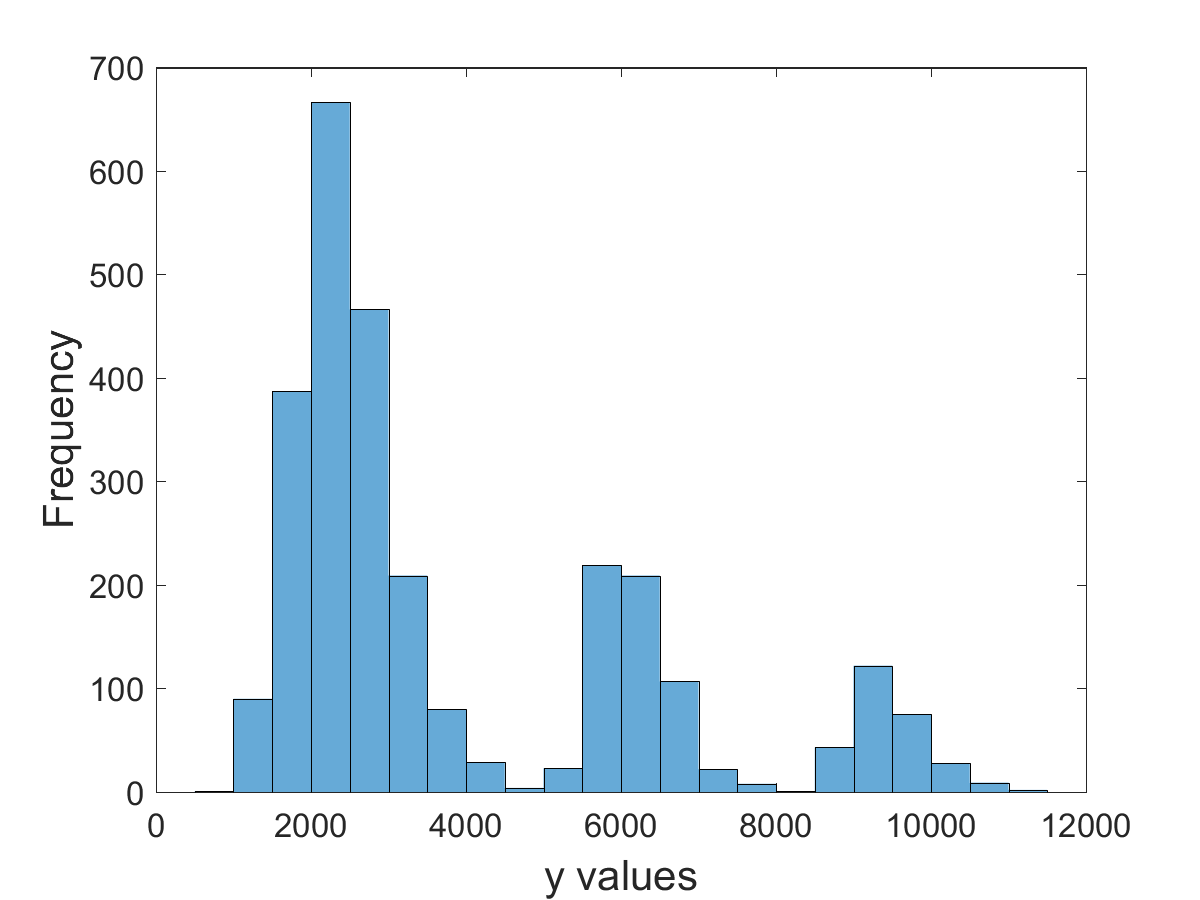
\includegraphics[width=2.2in]{figures/y_histogram.png}
	\caption{Histogram of $y$. We can see three bursts of data.}
	\label{fig:reg_yHistogram}
\end{figure}

We also computed the eigenvalues of the matrix $X^T X$. As ten eigenvalues are smaller than $10^{-10}$, we will need to transform $X$ to remove dimensions corresponding to those small eigenvalues or to use methods such as ridge regression to lift them. 

\begin{figure}[!h] % !t
\center
\subfigure[$y$ in function of $55^{th}$ dimension of $X$.]{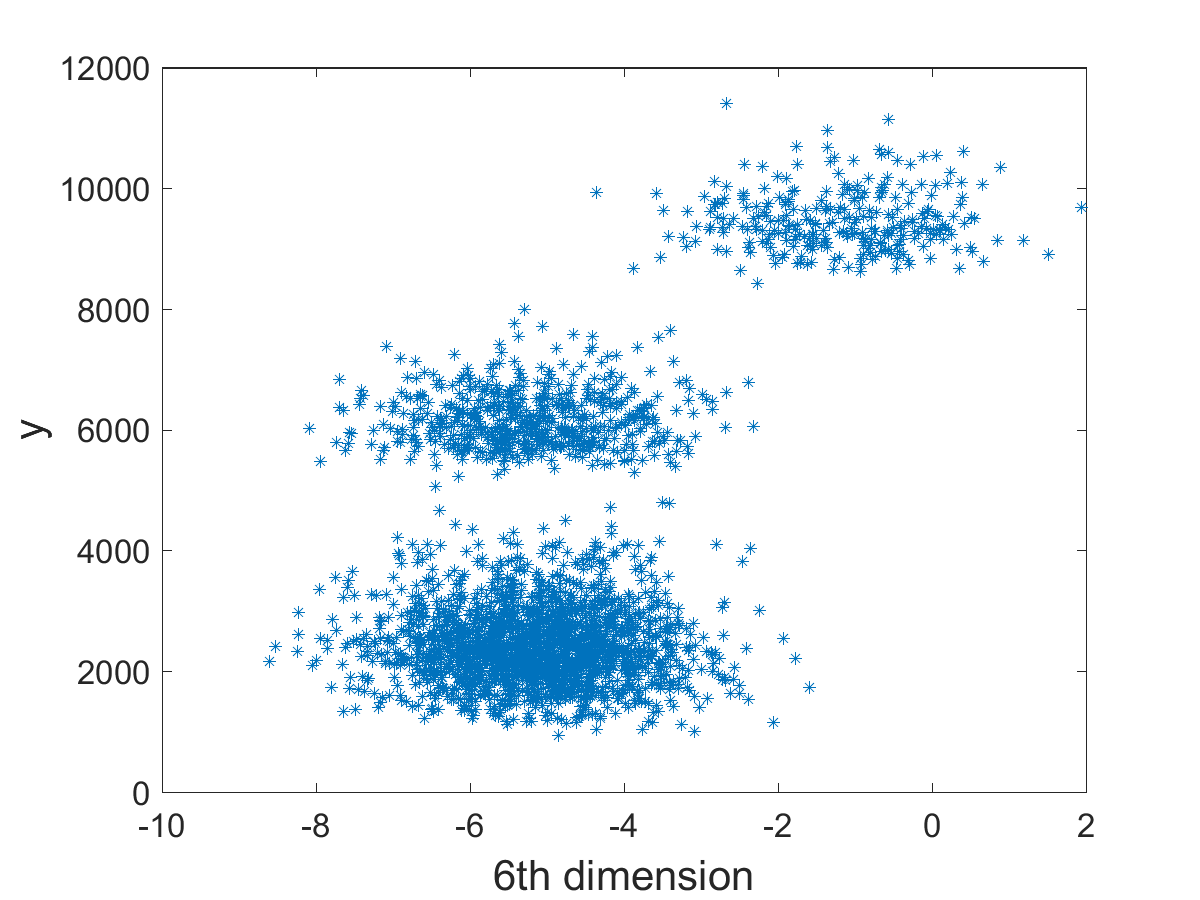
\includegraphics[width=2.2in]{figures/dim6.png} \label{fig:reg_dim6}}
\hfill
\subfigure[$y$ in function of $6^{th}$ dimension of $X$.]{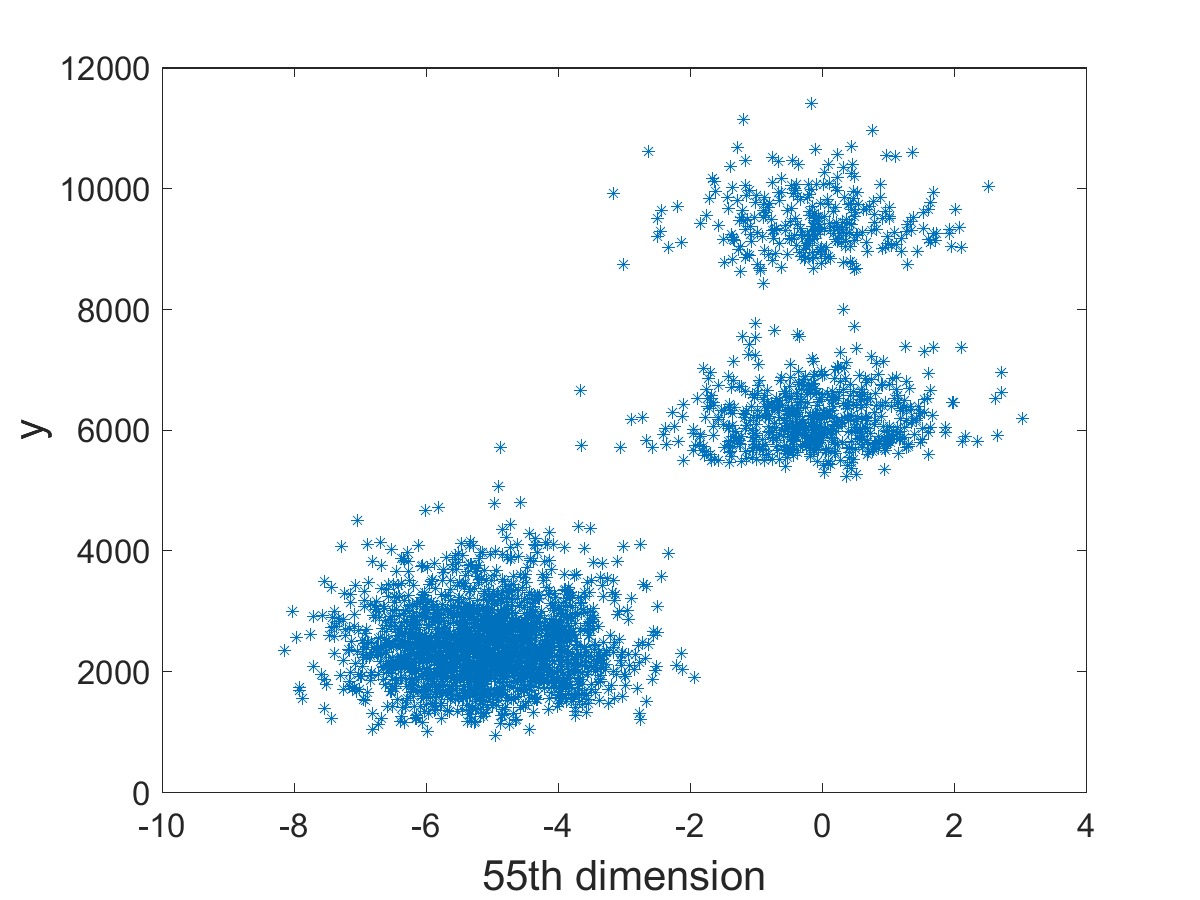
\includegraphics[width=2.2in]{figures/dim55.png} \label{fig:reg_dim55}}
\caption{Graphs of $y$ in function of the input dimensions most correlated with the output.}
\end{figure}

\subsection{Clustering}
We used k-means clustering to separate our data during the training part. The clustering is always done before normalising the data.
As the data are not equally shared between the three clusters, we first compute a clustering with $k=2$ clusters using $y$ and the most correlated dimension of $X$ with $y$ to compute the distance between each data-point and centre. In a second step, we keep only the data classified in the sparse cluster to make a second clustering with $k=2$ using $y$ and the second most correlated dimension of $X$. Figure ~\ref{fig:reg_clustersTrain} shows an example of clusters obtained after the training.

\begin{figure}[!h] % !t
	\center
	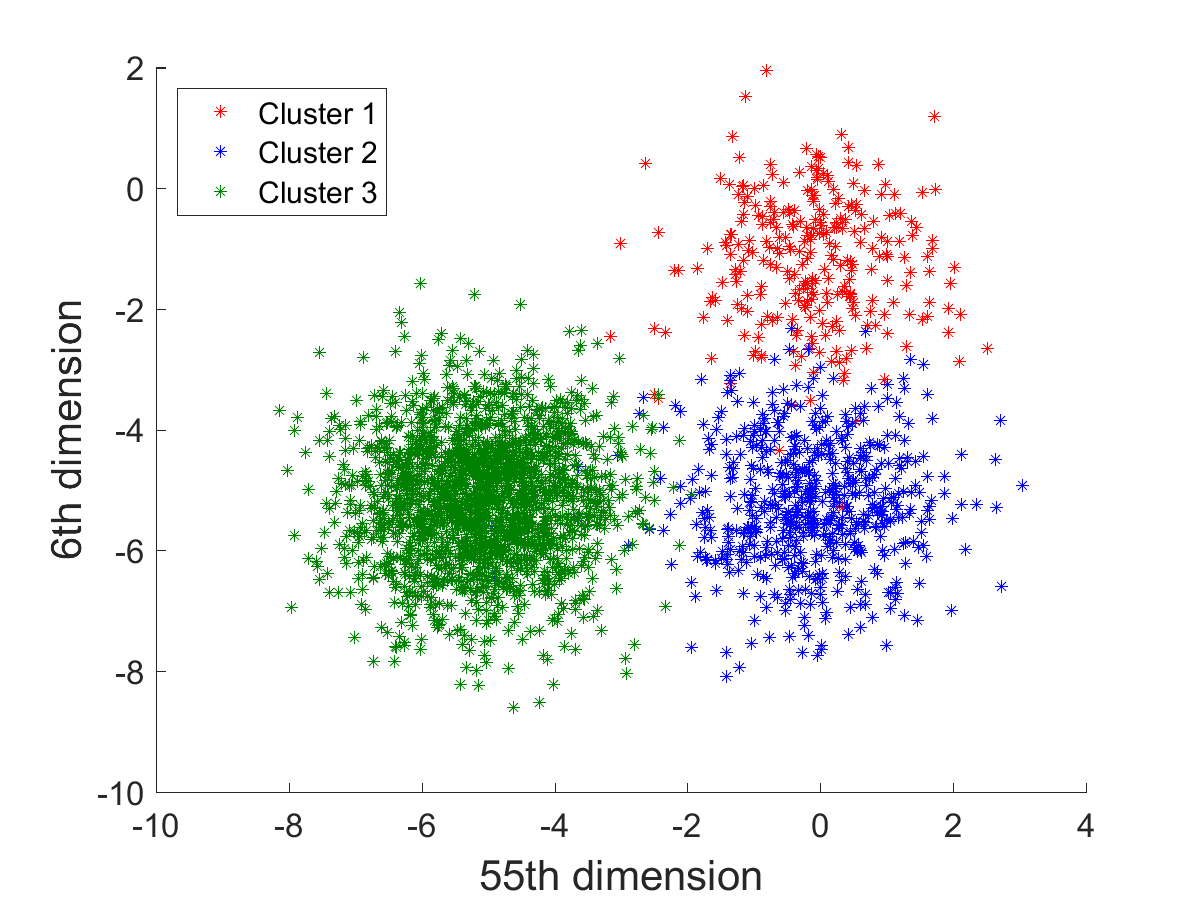
\includegraphics[width=2.2in]{figures/clusters_train.png}
	\caption{Clusters obtained along the two most correlated dimensions. We can see three clearly delimited groups of data.}
	\label{fig:reg_clustersTrain}
\end{figure}

In order to ensure a reliable clustering, we do not initialise the centres randomly. During the initialisation, we sort the data-points by their norm and separate the sorted list in $k$ chunks, where $k$ is the given number of clusters. The mean along each dimension is then calculated for each chunk giving the initial centres for the clusters.

During the test part, we follow the same principle. The most correlated dimension of $X$ found during the training part is used to find the closest centre and the second most correlated dimension is then used to divide the data classified in the sparse cluster in two sub-clusters.

Figure ~\ref{fig:reg_clustersTest} shows an example of k-means clustering for test data.

\begin{figure}[!h] % !t
	\center
	\subfigure[First k-means applied along the most correlated dimension of $X$ with $y$.]{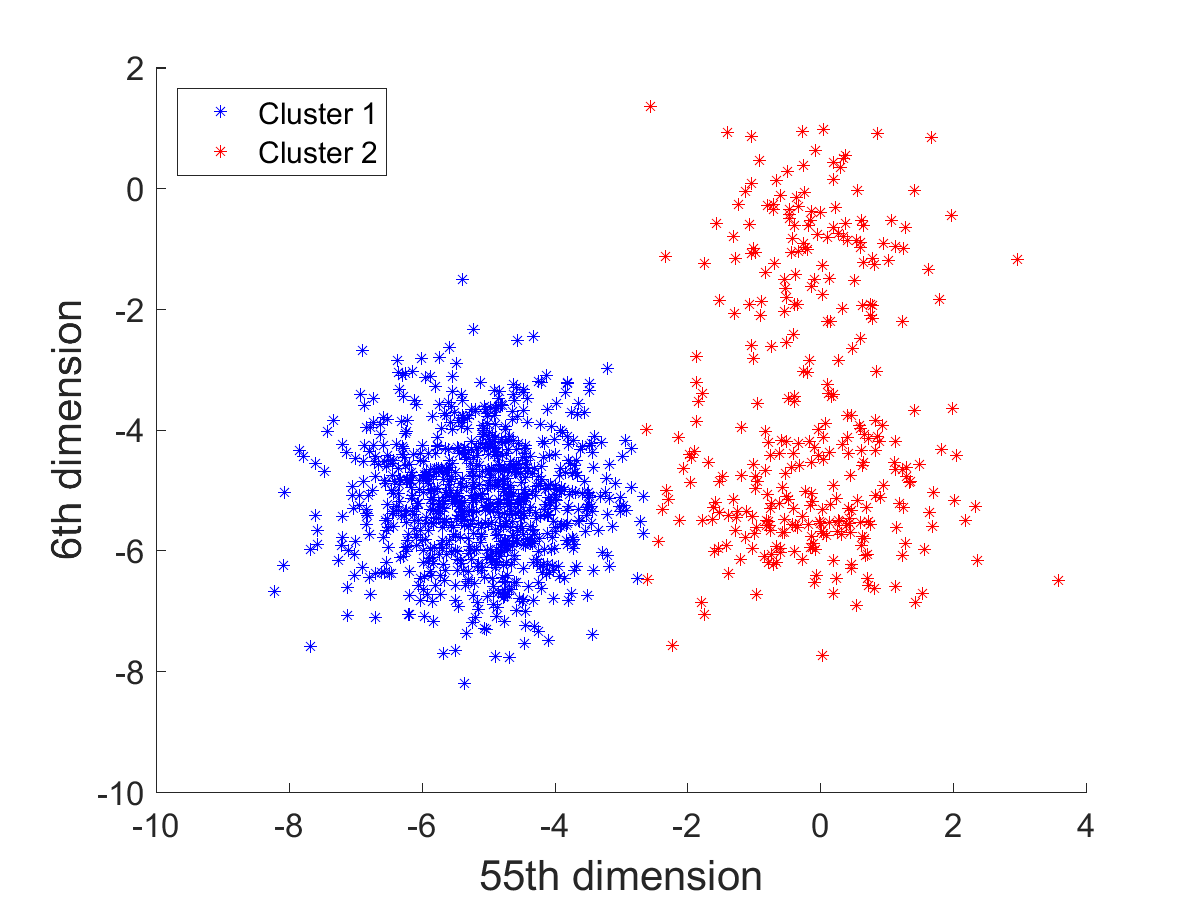
\includegraphics[width=2.2in]{figures/clusters_phase1.png} \label{fig:reg_clustersTest1}}
	\hfill
	\subfigure[Second k-means applied along the second most correlated dimension of $X$ with $y$.]{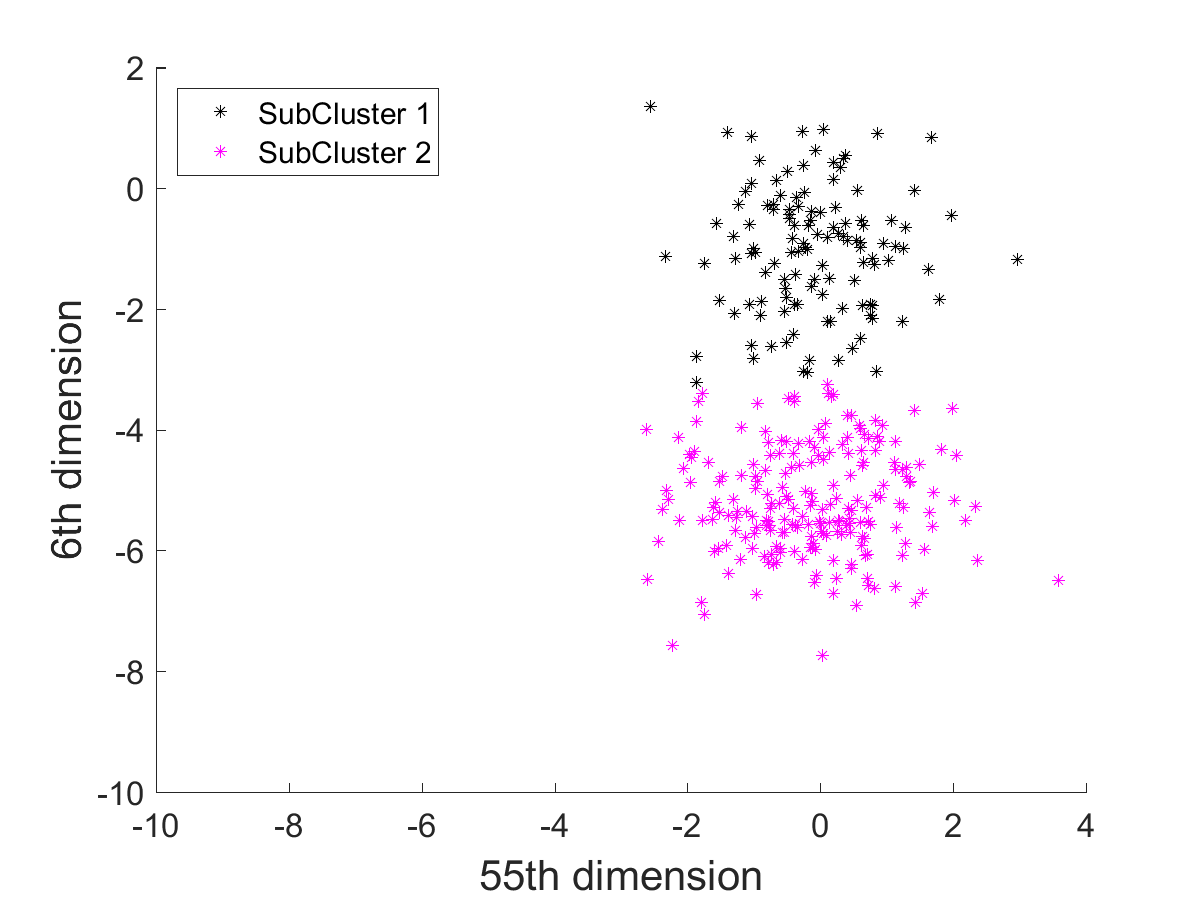
\includegraphics[width=2.2in]{figures/clusters_phase2.png} \label{fig:reg_clustersTest2}}
	\caption{Steps of k-means clustering for test-data.}
	\label{fig:reg_clustersTest}
\end{figure}

\subsection{Feature transformations}
After the separation in cluster, each group of train-data is treated separately. For each cluster, the dimensions of $X$ and $y$ are normalised to have zero-mean and unitary standard deviation. We also implemented a method to fix the outliers and a PCA to improve our predictions. 

We defined as outliers the data-points for which some elements of one or more real-valued dimensions are further than 3 standard deviations from the mean. As our data were normalised, all non-categorical element higher than 3 were considered as outlier elements. To fix the outliers, value $3$ (or $-3$) was assigned to those elements. Fixing the outliers with this methods allows us to avoid errors in prediction models due to false-classified data.

The PCA is applied only on the real-valued dimensions. It projects our input data in a new coordinate system based on the covariance between dimensions. It allows us to reduce the dimensionality of our data in this new space by removing the dimensions with eigenvalues lower than a defined value. We choose this value equal to $1$ as eleven dimensions have eigenvalues in the order of $10^{-10}$ and all others are higher than $10$. The data are then projected back in the initial coordinate system. In our case, the PCA reduce our input data by eleven dimensions.

After the clustering of test-data, each group is also treated separately. The data are first normalised given the means and standard deviations computed during the training. The outliers are then fixed and PCA is applied by projecting the data with the eigenvectors computed during the training part.

\subsection{Least-Squares and Ridge Regression}
We applied least-squares, least-squares with gradient descent and ridge regression to our dataset. Using PCA allows us to solve the problem of ill-conditioned matrix, so that we can use the three methods mentioned above. The ridge regression is the only method that can be used without reducing the dimensionality of the input data.

We computed the RMSE for each model with and without the categorical dimensions of X. As removing those dimensions does not change significantly the error, we decided to compute the regression only with the 60 real-valued dimensions.

Figure ~\ref{fig:reg_alphaRMSE} shows the train and test RMSE for a step size $\alpha$ varied from $10^{-3}$ to $10^{-0.5}$ with $20$ points in between. The convergence condition was reached when the variation of $\beta$ between two iterations was lower than $1.5 \alpha$. Cross-validation was made using $66 \% $ of the data as train data and the rest as test data. We observe that the bias is higher and the variance globally lower for small values of $\alpha$. The RMSE is optimal for $\alpha \approx 0.2$. With higher $\alpha$ values, gradient descent is not able to converge and the error goes to $\infty$.

\begin{figure}[!h] % !t
	\center
	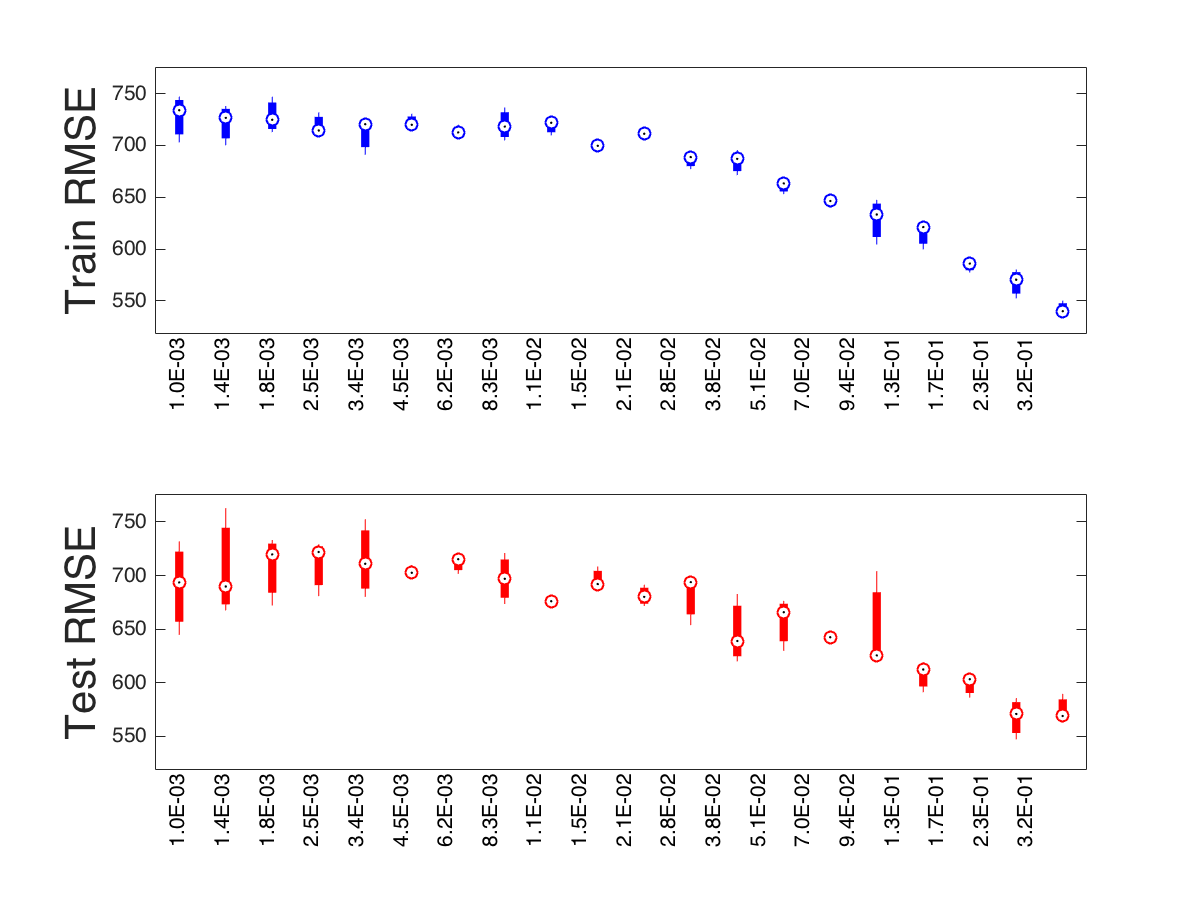
\includegraphics[width=3in]{figures/alphaRMSEBox.png}
	\caption{Ridge regression for a $66 \%$ - $33 \%$ split with 3 iterations for each $\lambda$.}
	\label{fig:reg_alphaRMSE}
\end{figure}

Figure ~\ref{fig:reg_lambdaRMSE} shows the train and test RMSE for $\lambda$ varied from $10^{-3}$ to $10^{7}$ with $60$ points in between. Cross-validation was made using $66 \% $ of the data as train data and the rest as test data. We can see that $\lambda$ should be chosen between $0$ and $100$ to have the best prediction and that $\lambda$ higher than $1000$ increases the RMSE and the model under-fits. For high $\lambda$ values, the model and estimation bias are increased as their variance is reduced.

\begin{figure}[!h] % !t
	\center
	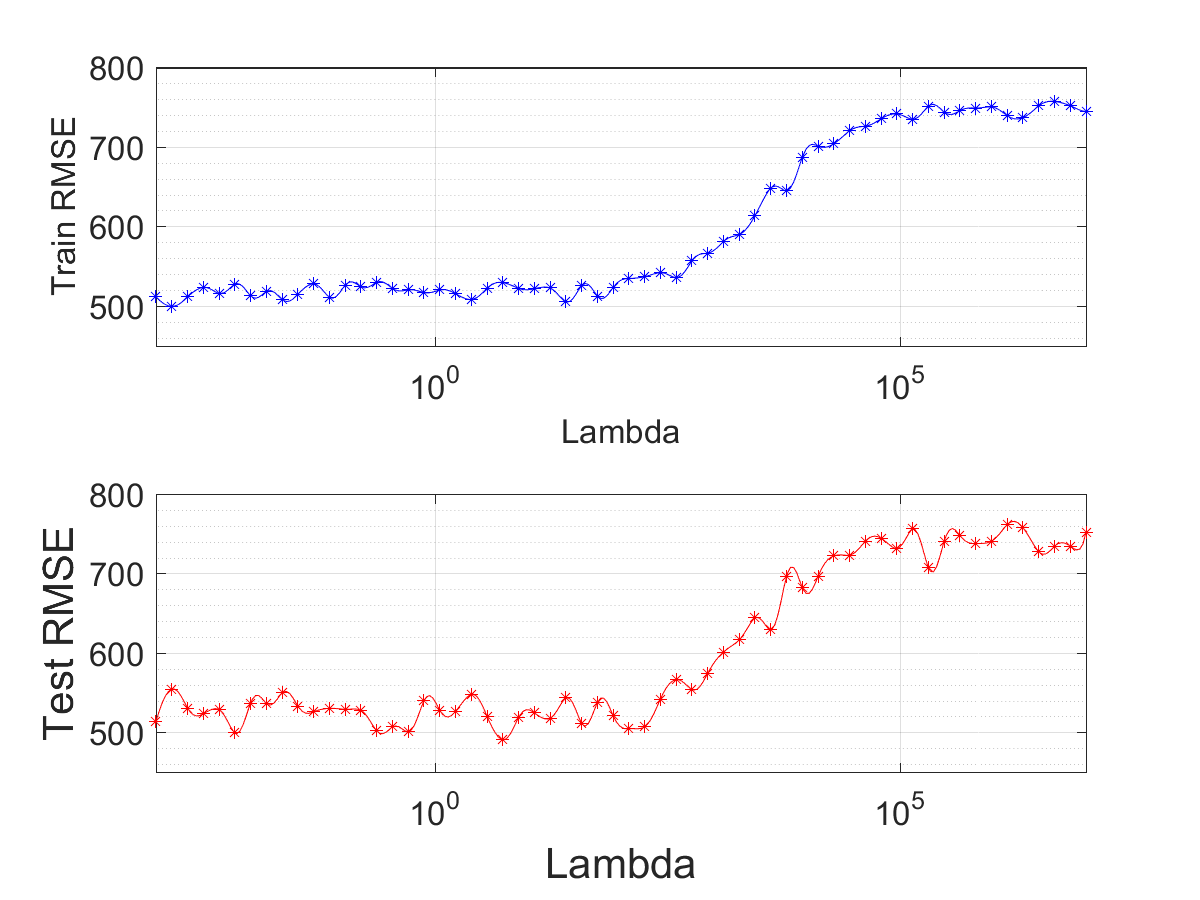
\includegraphics[width=3in]{figures/lambdaRMSE.png}
	\caption{Ridge regression for a $66 \%$ - $33 \%$ split with 3 iterations for each $\lambda$.}
	\label{fig:reg_lambdaRMSE}
\end{figure}

Figure ~\ref{fig:reg_compareMethods} compares three regression methods with $\alpha = 0.3$ for the gradient descent and $\lambda = 100$ for ridge regression. It is important to note that some outliers (11 for the train, 17 for the test) of least-squares method are not visible in this graph, as their RMSE is higher than $10^4$.

\begin{figure}[!h] % !t
	\center
	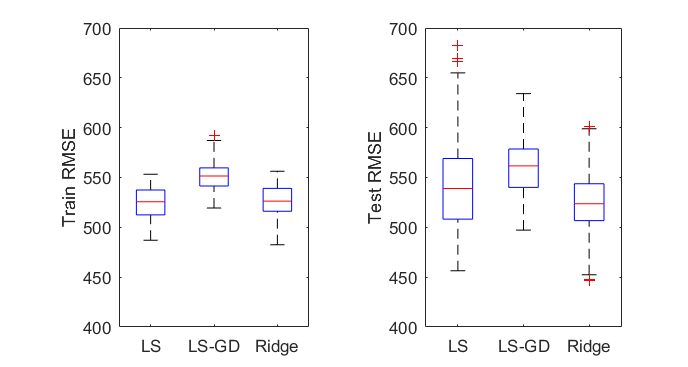
\includegraphics[width=3in]{figures/comparisonReg.png}
	\caption{Boxplots of train and test RMSE for least-squares (LS), least-squares with gradient descent (LS-GD) and ridge regression (Ridge).}
	\label{fig:reg_compareMethods}
\end{figure}

The median train/test RMSE are respectively equal to $526/539$, $551/562$ and $526/524$ for least-squares, least-squares GD and ridge regression. We observe that least-squares GD has a high bias and a low variance compared to least-squares that has a lower bias and a higher variance. 

\section{Classification}
\subsection{Data Description}
Our classification-data contains $N=1500$ train-examples and $N=1500$ test-data. The train-data are composed of input and output variables $X$ and $y$. Each input $x_n$ has a dimensionality $D=37$ with 32 real-valued variables, 2 binary variables, 3 categorical variables with 5 categories. The output is a binary variable equal to $1$ or $-1$. The output of our test-data is not observed. Our goal is then to predict $y$ for all test-examples and to give an approximation of the test-error.

\subsection{Data Visualization and Cleaning}
To visualise our data, we plotted histogram of $X$ dimensions. The input data is again not centred, so that we need to normalise it.

Figures ~\ref{fig:class_dim23} and ~\ref{fig:class_dim35} show respectively the histogram of the $23^{th}$ and the $35^{th}$ variable of $X$. We see that the distribution is composed of a high peak and a Gaussian distribution. We observed that most of the real-valued dimensions have similar distributions and that data-points belonging to the peak or to the Gaussian in one dimensions are contained in the same part of the distribution in other dimensions. Moreover, the binary value of the $20^{th}$ dimension is different for data-points in the peak or in the Gaussian, so that we can use this dimension to separate the input data in two clusters.

We also computed the eigenvalues of the matrix $X^{T}X$. As the smaller eigenvalue is equal to $58.4$, the matrix is full-rank and we do not need to use methods to lift the eigenvalues.

\begin{figure}[!h] % !t
	\center
	\subfigure[Histogram of the $23^{th}$ dimension of $X$.]{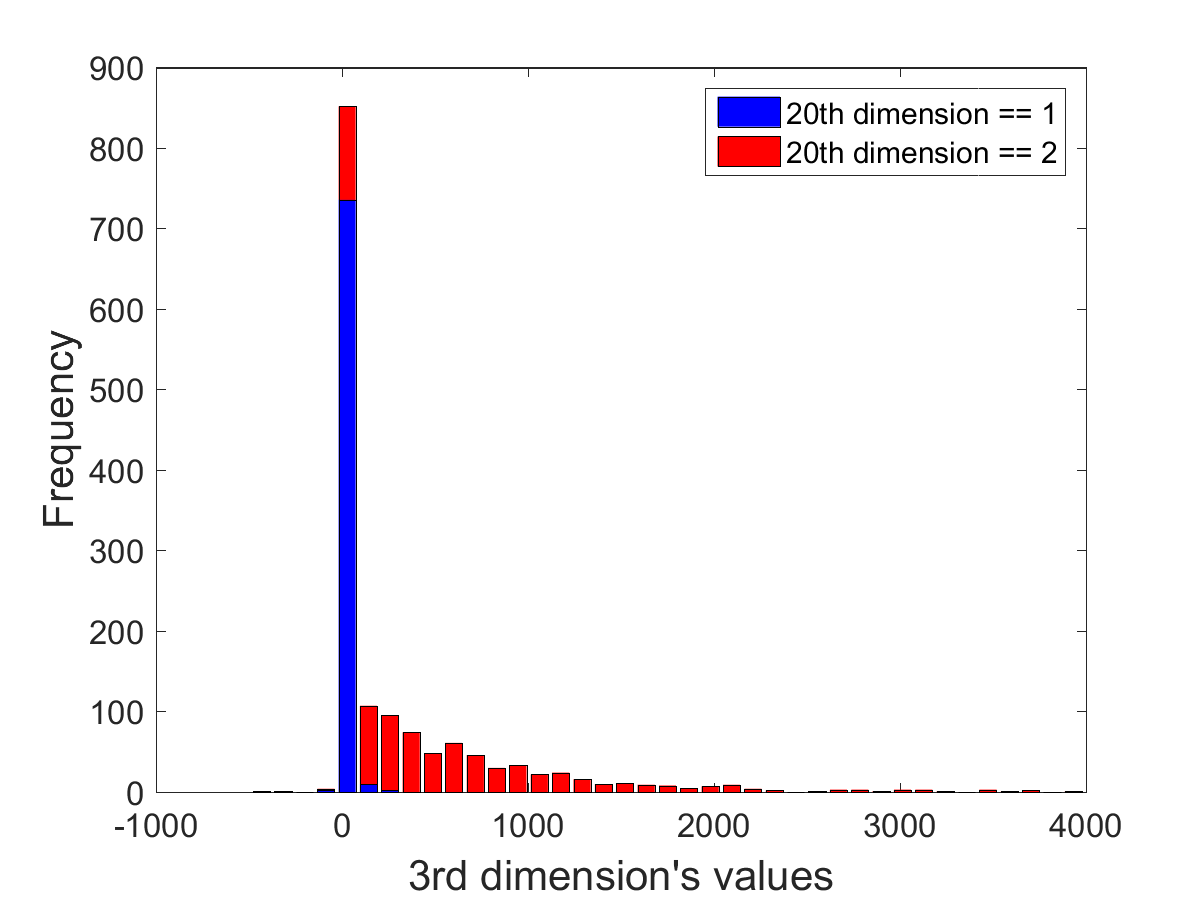
\includegraphics[width=2.6in]{figures/dim23.png} \label{fig:class_dim23}}
	\hfill
	\subfigure[Histogram of the $35^{th}$ dimension of $X$.]{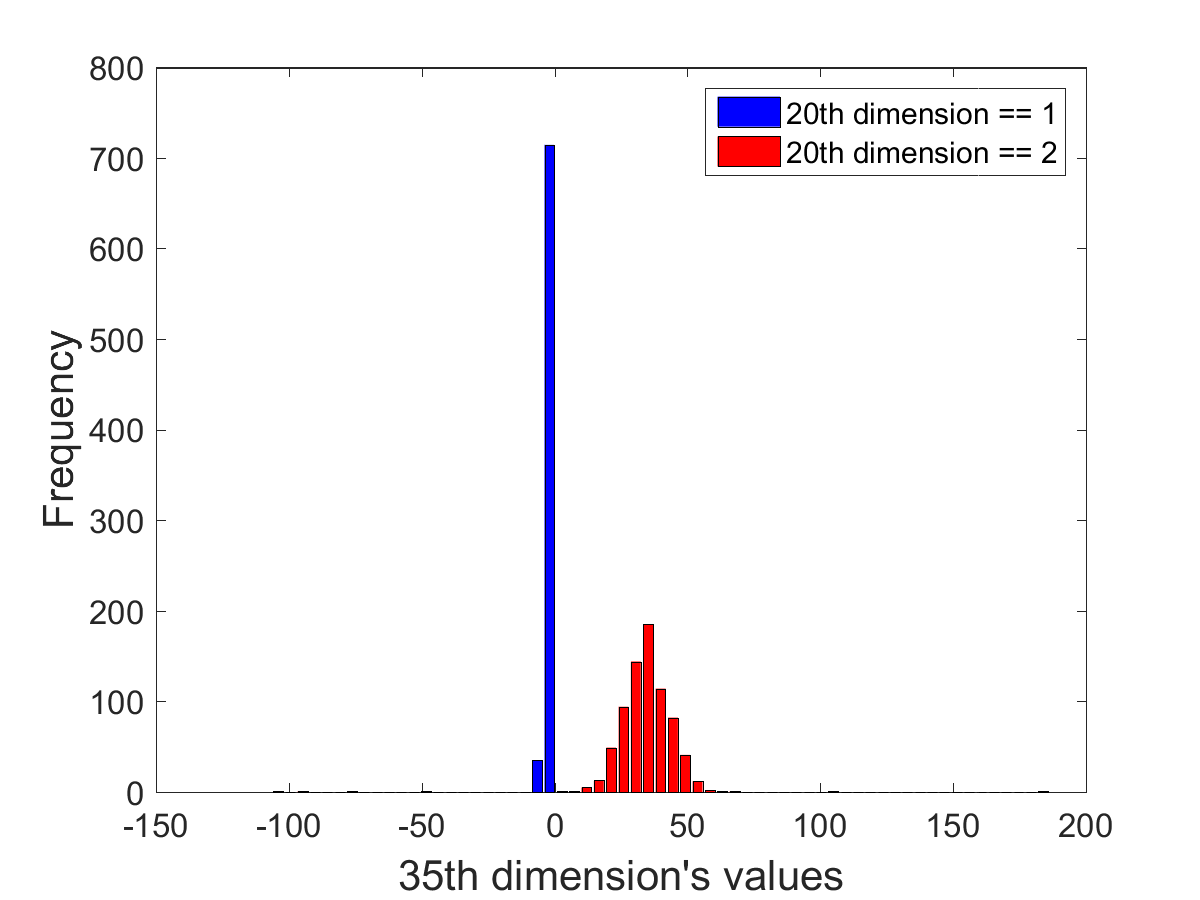
\includegraphics[width=2.6in]{figures/dim35.png} \label{fig:class_dim35}}
	\caption{Example of histogram to show the distribution of $X$ dimensions. We can see that each distribution is composed of a peak in blue and of a Gaussian in red, separable given the $20^{th}$ variable.}
\end{figure}

\subsection{Feature Transformations}
The train-data are first separated in two clusters given the value of the 20th dimension of $X$. Each group of data are then treated separately. The real-valued variables of $X$ are first normalised to have zero-mean and unitary standard deviation. We also implemented a method to remove the outliers.

We defined as outliers the data-points for which at least one element of a real-valued dimension is further than 3 standard deviations from the mean. In this case, the data point is removed from the training set. 

After the clustering of the test-data, each group is also treated separately. The real-valued input data are normalised given the means and standard deviations computed during the training.

\subsection{Logistic Regression}
We applied logistic regression and penalised logistic regression on our dataset. Both regressions were implemented with Newton's method. To improve the convergence, the step size was adapted at each time step to be proportional to the log likelihood such that $\alpha = log(\ell) * 10^{-4}$. The convergence criterion was reached when the difference between $\beta$ between two consecutive iterations was lower than $0.001$.

Figure TODO shows the train and test TODO ERROR for $\lambda$ varied from

\section{Summary}
In this report, we analyse a regression and a classification dataset. We used k-means clustering and PCA to preprocess the regression data. We found that least-squares, least-squares with gradient descent and ridge regression TO DO.

We separated the classification data using a binary dimension that classify the data in two different distributions along the variable of the input data. We found that TODO.


\subsubsection*{Acknowledgments}
...

\subsubsection*{References}

\end{document}
